\documentclass[5p,times]{elsarticle}

\usepackage{lipsum}

%% For including figures, graphicx.sty has been loaded in
%% elsarticle.cls. If you prefer to use the old commands
%% please give \usepackage{epsfig}

%% The amssymb package provides various useful mathematical symbols
\usepackage{amssymb}
%% The amsthm package provides extended theorem environments
%% \usepackage{amsthm}

% Please add the following required packages to your document preamble for tables:
\usepackage[utf8]{inputenc}
\usepackage[spanish]{babel}
\usepackage{booktabs}
\usepackage{float}
\usepackage{graphicx}
\RequirePackage[colorlinks,citecolor=blue,urlcolor=blue]{hyperref}
%% Caption package for caption in figures and tables
\usepackage{caption}

%\journal{Nuclear Physics B}

%% Remove the line "Preprint submitted to Elsevier"
\makeatletter
\def\ps@pprintTitle{%
	\let\@oddhead\@empty
	\let\@evenhead\@empty
	\let\@oddfoot\@empty
	\let\@evenfoot\@oddfoot
}

\makeatother

\begin{document}


\begin{frontmatter}

\title{Diseño de experimento para el problema de empaquetamiento óptimo de politopos convexos definidos por sus vérticess}


\author{Alberto Martínez-Noa}
\address{Facultad de Ingeniería Mecánica y Eléctrica,
Universidad Autónoma de Nuevo León}
\ead{alberto.martineznn@uanl.edu.mx}

\begin{abstract}
En los problemas de C\&P contamos con un conjunto de elementos pequeños llamados carga que deben ser dispuestos o asignados a uno o varios objetos de gran tamaño llamados contenedores, y se debe cumplir la no superposición entre elementos pequeños y que dichos conjuntos de elementos no excedan las dimensiones del contenedor al cual han sido asignados. Dichos problemas se clasifican como NP-duros \cite{FOWLER1981133} debido a su complejidad computacional. 
En este Trabajo se presenta un diseño de experimento para un modelo no lineal de empaquetamiento con un enfoque lagrangiano en las condiciones de no intersección que analiza las figuras por sus vértices. En el mismo se analizan como influyen los factores (tipo de figura, cantidad de figura y tipo de contenedor) en la densidad de empaque con el empleo de este modelo.
 
\end{abstract}

\begin{keyword}
	Empaquetamiento óptimo \sep ANOVA \sep diseño de experimento\sep pruebas no perimétricas. 
	%% keywords here, in the form: keyword \sep keyword
	
	%% PACS codes here, in the form: \PACS code \sep code
	
	%% MSC codes here, in the form: \MSC code \sep code
	%% or \MSC[2008] code \sep code (2000 is the default)
	
\end{keyword}

\end{frontmatter}

\section{Introduction}

   En los problemas de C\&P contamos con un conjunto de elementos pequeños llamados carga que deben ser dispuestos o asignados a uno o varios objetos de gran tamaño llamados contenedores, y se debe cumplir la no superposición entre elementos pequeños y que dichos conjuntos de elementos no excedan las dimensiones del contenedor al cual han sido asignados. Dichos problemas se clasifican como NP-duros \cite{FOWLER1981133} debido a su complejidad computacional.

   Este trabajo de investigación se centrará en la resolución del problema de empaquetamiento de un surtido arbitrario de elementos pequeños convexos en un único contenedor convexo de dimensiones variables que se puede tratar como el problema de dimensión(es) abierta(as) (ODP, por sus siglas en inglés).

   El problema de dimensión abierta es un problema en el cual, el conjunto de elementos pequeños debe ser acomodado completamente dentro de un objeto grande o contenedor. El objeto grande, posee al menos una dimensión puede considerarse variable. En otras palabras, este problema implica una decisión sobre la fijación de las extensiones en las dimensiones variables de los objetos grandes, así como el valor de la entrada u otra medida como longitud, tamaño o volumen se deben minimizar \cite{WASCHER2007}.
   
   Este trabajo presenta un diseño de experimento para un modelo no lineal con un enfoque lagrangiano para las condiciones de no intersección que analiza las figuras por sus vértices. La definición de los elementos a empaquetar por sus vértices no ha sido tratada en la literatura revisada \cite{litvinchevlagrangian}. 

	
	El presente trabajo está estructurado de la siguiente forma. En la Sección \ref{Section2} se muestra una descripción de las instancias. A continuación, en la Sección \ref{Section3}, se presenta el diseño de experimento. En la sección \ref{Section4} se realiza un análisis estadísticos de los resultados para el contenedor tipo sección-circular. La sección \ref{Section5} analiza los resultados del contenedor circular. En la sección \ref{Section6} se muestra los resultados del análisis por tipo de contenedor, y finalmente en la sección \ref{Section7} se presentan las conclusiones alcanzadas.
	
\section{Descripción de las instancias}\label{Section2}
	
	Las instancias analizadas en esta investigación fueron creadas, con un generador de instancias programado en lenguaje Python \cite{Phy}, con fin de validar el modelo propuesto. En el cuadro \ref{tab:instancias} se muestra la cantidad de instancias para los dos tipos de contenedores analizados (sección-circular, circular). Las instancias para cada una de las figuras solamente varían en el número de elementos (5, 6, 7, 8, 9, 10, 15, 20, 25, 30) a empacar. En el caso de los pentágonos existen diez instancias para los regulares (pentágonos$_r$) y la misma cantidad de para los irregulares (pentágonos$_i$).   
	 
	 % Table generated by Excel2LaTeX from sheet 'Hoja1'
\begin{table}[H]
  \centering
  \caption{Cantidad de instancias por figura}

    \begin{tabular}{lc}
    \toprule
      Figuras &  Cantidad de instancias\\
    \midrule
         triángulos & 10    \\
         rectángulos& 10    \\
         cuadrados & 10   \\
       pentágonos$_r$ & 10    \\
           pentágonos$_i$ & 10     \\
           cuadriláteros mixtos  & 10  \\
          hexágonos & 10    \\
        tetraedros & 10   \\
          
    \bottomrule
    \end{tabular}%

  \label{tab:instancias}%
\end{table}%

\section{Diseño de experimento}\label{Section3}
	
	En esta experimentación se contemplan dos tipos de contenedores y siete tipos de figuras diferentes a empacar con 10 tamaños de instancias diferentes. Por lo que se utiliza un diseño factorial completo con tres factores de control por tratamiento por lo que se tiene 140 tratamientos. Dichos factores de control son: 

\begin{itemize}
    
    \item Tipo de contenedor de dos niveles (sección-circular, circular),
    \item Tipos de figuras de siete niveles (triángulos, cuadrados, rectángulos, pentágonos (regulares e irregulares) y hexágonos, cuadriláteros mixtos), 
    \item Cantidad de elementos de la instancia (5, 6, 7, 8, 9, 10, 15, 20, 25, 30).
\end{itemize}

\section{Análisis estadístico contenedor tipo sección-circular}\label{Section4}

El objetivo de esta es investigación es determinar si los tipos de figuras, la cantidad de estas y el tipo de contenedor influyen en el porciento de ocupación de los elementos en el contenedor. Para cumplir dicho objetivo realizaremos un análisis estadístico de los datos, dividiéndolos por tipos de contenedor.
 
Para el analizar de los resultado se pretende usar un análisis de varianza (ANOVA) unidireccional, donde se toma como variable dependiente el porciento de ocupación y como factores el tipo de figura, la cantidad de figuras a empaquetar en cada caso.
	
Antes de realizar el ANOVA, se debe comprobar tres supuestos: las poblaciones (distribuciones de probabilidad de la variable dependiente correspondiente a cada factor) son normales, las K muestras sobre las que se aplican los tratamientos son independientes y que las poblaciones tienen igual varianza (homoscedasticidad) \cite{Anl}.

Para el primer supuesto se realiza la prueba de Shapiro--Wilk, que calcula un W estadístico que prueba si una muestra aleatoria $x_{1}, x_{2}, ..., x_{n}$ proviene de una distribución normal. El resultado de esta prueba con un $\textbf{W}=0.966$ y un \textbf{valor $p$} = 0.055 mayor que $\alpha = 0.050$ muestra que no existe suficiente evidencia para rechazar la hipótesis nula, la cual plantea que la variable dependiente (densidad) sigue una distribución normal. Esto se puede afirmar con un intervalo de confianza del 95\%. En la figura \ref{fig:normal1} se muestra que todos los puntos caen aproximadamente a lo largo de la línea de referencia, podemos asumir la normalidad.
	\begin{figure}
				\begin{center}
					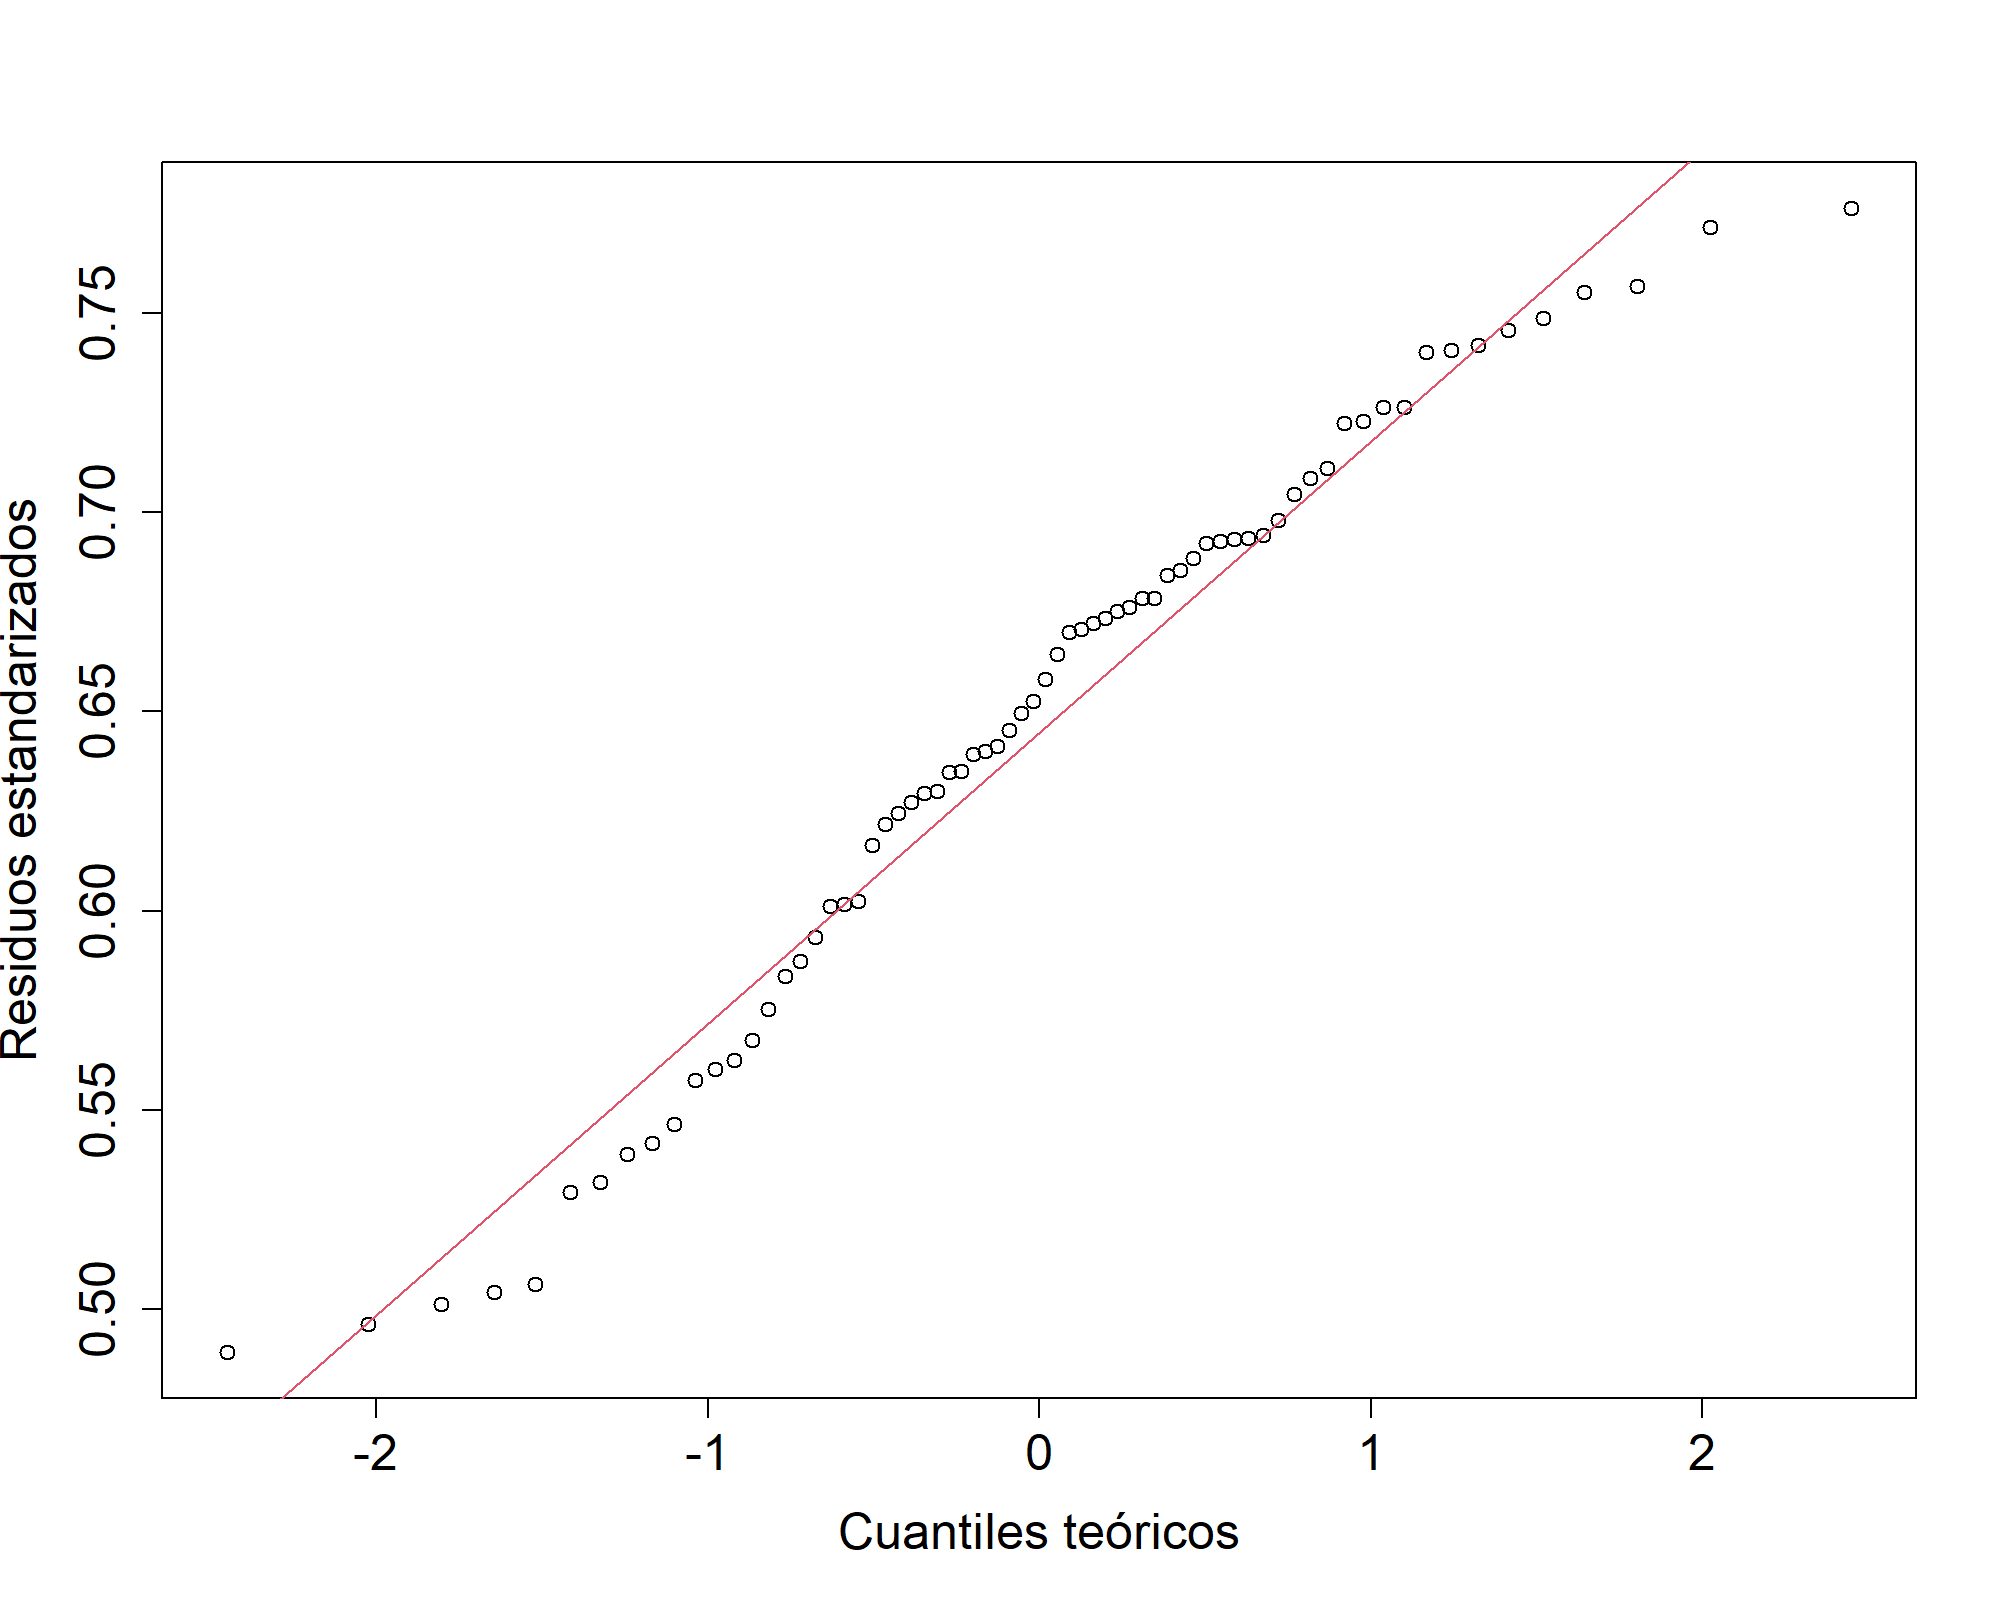
\includegraphics[scale=0.35]{figuras/sseccnormal.png}
					\captionof{figure}{Gráfica Q-Q normal para la variable densidad}
					\label{fig:normal1}
				\end{center}
			\end{figure}
			
Dado que los datos se encuentran en el límite para aceptar que se distribuye de forma normal, la prueba de Fisher y el de Bartlett no son recomendables. En su lugar es mejor emplear una prueba basada en la mediana prueba de Levene o prueba de Fligner-Killeen. En dicha prueba con $\chi^2$ = 5.319 y un \textbf{valor $p$} = 0.378 mayor que $\alpha = 0.050$ arroja que no existe suficiente evidencia para rechazar la hipótesis nula, por lo que variable dependiente (densidad) tiene homoscedasticidad con un intervalo de confianza del 95\%.

Divido a los resultados obtenidos anteriormente se puede utilizar un ANOVA unidireccional, donde se toma como variable dependiente la densidad y como factores el tipo de figura, la cantidad de figuras a empaquetar en cada caso.

Para el primer factor (Tipo de figura) se plantea la siguiente pregunta: ¿Existe diferencia entre el promedio de ocupación de los diferentes tipos de figuras? La respuesta a esta pregunta se obtiene al contrastar las siguientes hipótesis:
\begin{equation}
H_{0}:\mu_{1}=\mu_{2}=\mu_{3}=\mu_{4}=\mu_{5}=\mu_{6}    
\end{equation}
\begin{equation}
 H_{1}:\mu_{i}\neq\mu_{j}\quad \mbox{para alguna} \quad i\neq j
\end{equation}

 Con los valores del estadístico de prueba \textbf{F} = 1.030 y \textbf{valor $p$} = 0.305 mayor que $\alpha = 0.050$ no se tiene evidencia suficiente para rechazar la hipótesis $H_{0}$ que nos indica que la no existencia diferencias estadísticas significativas entre los grupos con un intervalo de confianza del $95\%$. Esto se puede observar en la figura \ref{fig:boxplotssc1}.

	\begin{figure}
				\begin{center}
					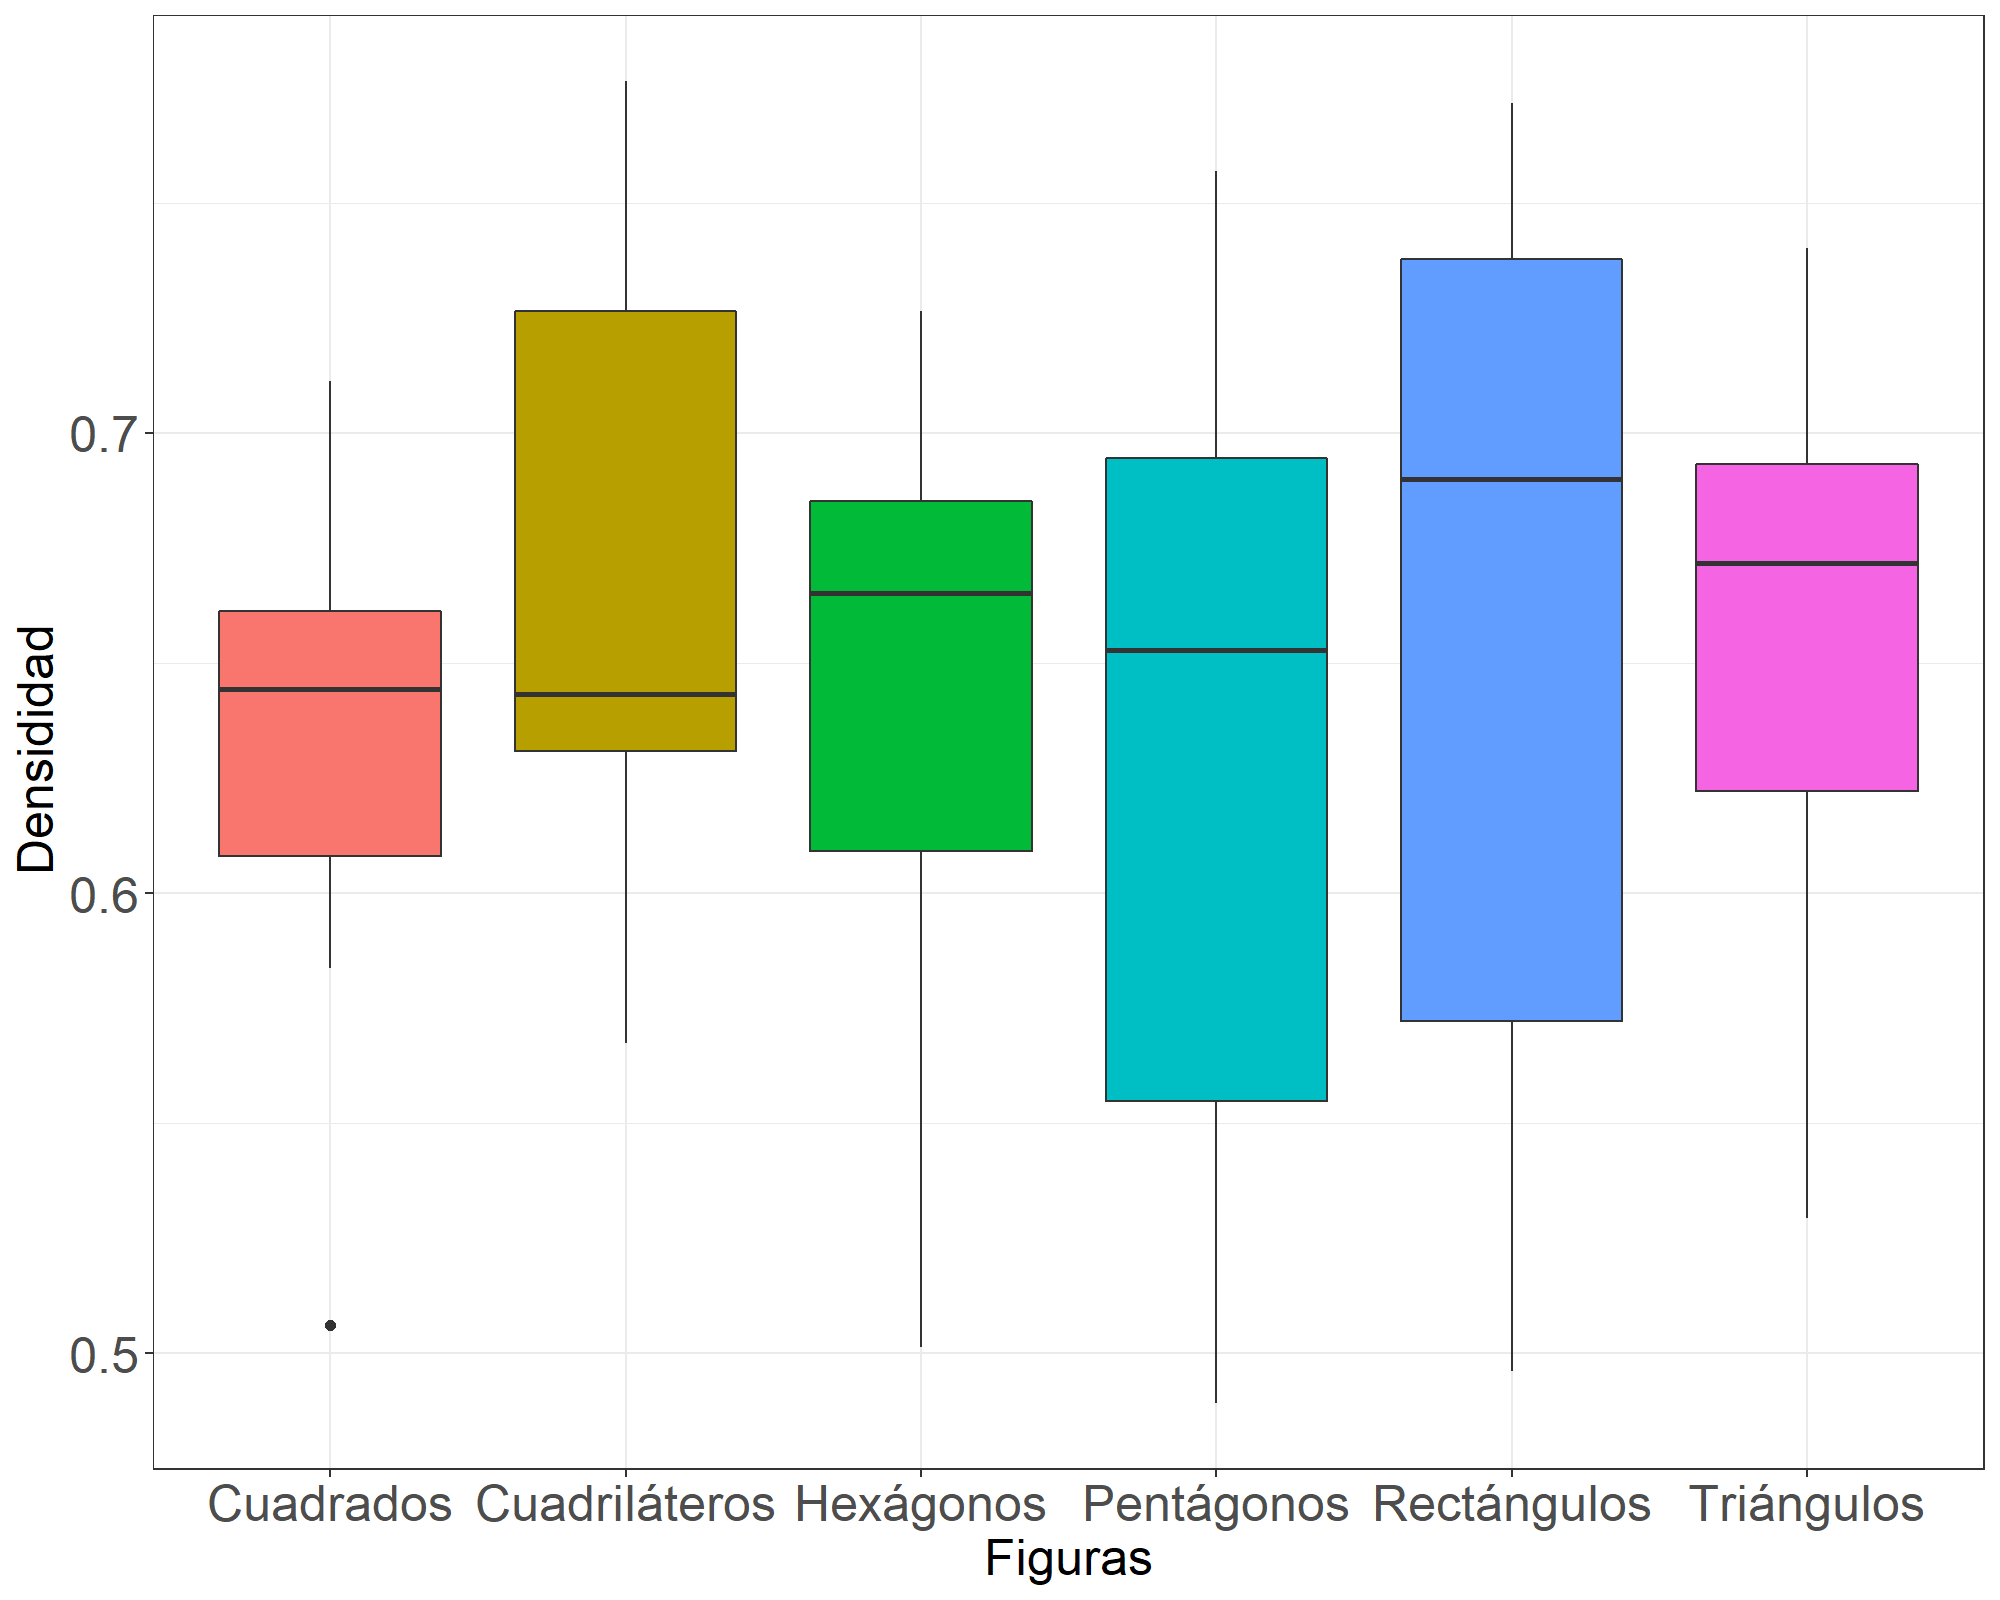
\includegraphics[scale=0.35]{figuras/Sseccboxplot.png}
					\captionof{figure}{Diagrama de caja y bigotes que relaciona los tipos de figuras y el \% de ocupación del contenedor}
					\label{fig:boxplotssc1}
				\end{center}
			\end{figure}
			
Análogamente al análisis del primer factor, se realiza la misma prueba para el factor de control cantidad de figuras. Con los valores del estadístico de prueba $\textbf{F} = 15.380$ y \textbf{valor $p$} = 0.000 menor que $\alpha = 0.050$, se tiene evidencia suficiente para rechazar la hipótesis $H_{0}$ ya que existe diferencias estadísticas significativas al menos entre algunos de los grupos con un intervalo de confianza de un $95\%$, esto se aprecia en la figura \ref{fig:boxplotssc2}. 

	\begin{figure}
				\begin{center}
					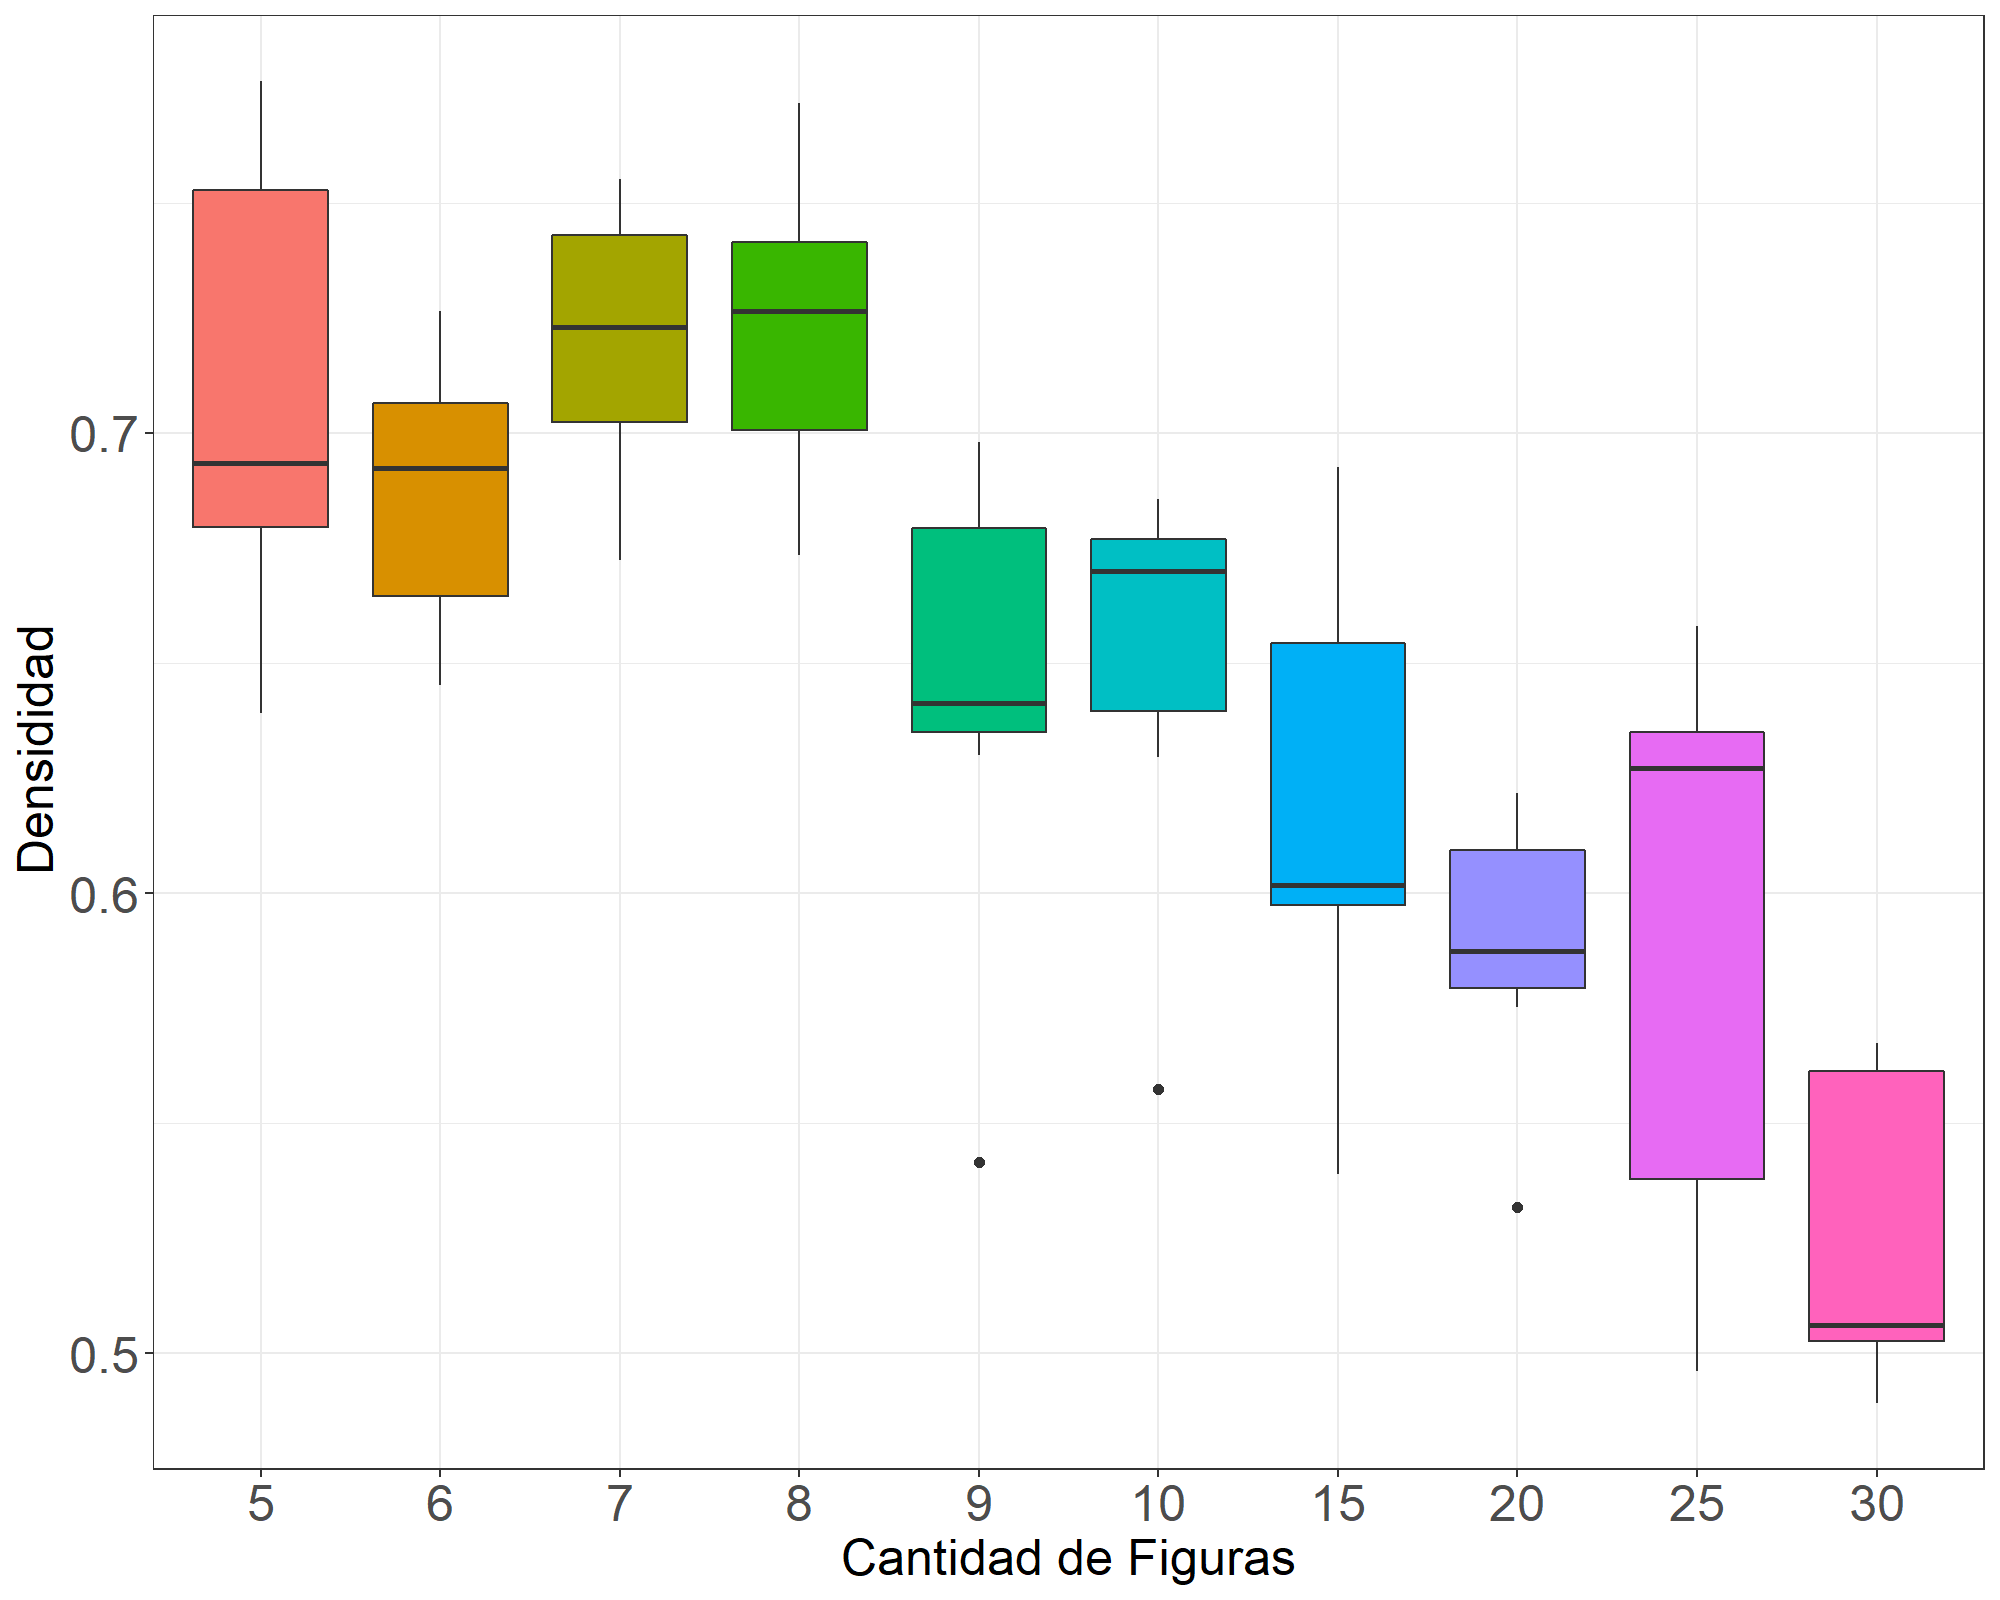
\includegraphics[scale=0.35]{figuras/Sseccboxplotcant.png}
					\captionof{figure}{Diagrama de caja y bigotes que relaciona la cantidad de figuras y el \% de ocupación del contenedor}
					\label{fig:boxplotssc2}
				\end{center}
			\end{figure}
			
El ANOVA no ofrece información suficiente para señalar entre que grupos existe la diferencia. Por lo que se aplica una prueba Tukey HSD (\textit{del inglés honestly significant difference}) que muestra las diferencias entre las medias de los grupos. los resultados de la prueba arrogan que se rechaza la hipótesis en los casos de pareo de la instancia de tamaño (10--30, 15--30, 15--5, 15--7, 15--8, 20--5, 20--6, 20--7, 20--8, 25--5, 25--6, 25--7, 25--8, 30--5, 30--6, 30--7, 30--8, 30--9 y 9--8), dado que los \textbf{valores $p$} son menores que $\alpha = 0.050$, como se aprecia gráficamente en la figura \ref{fig:tykey1}.

Los resultados obtenidos en esta sección nos indican que para el caso del contenedor tipo sección-circular el tipo de figura  a empacar no influye significativamente en el porciento de ocupación del contenedor, por otro lado la cantidad de elementos a empacar si influye en la ocupación del contenedor y se observa que a mayor número de elementos la densidad disminuye.

	\begin{figure}
				\begin{center}
					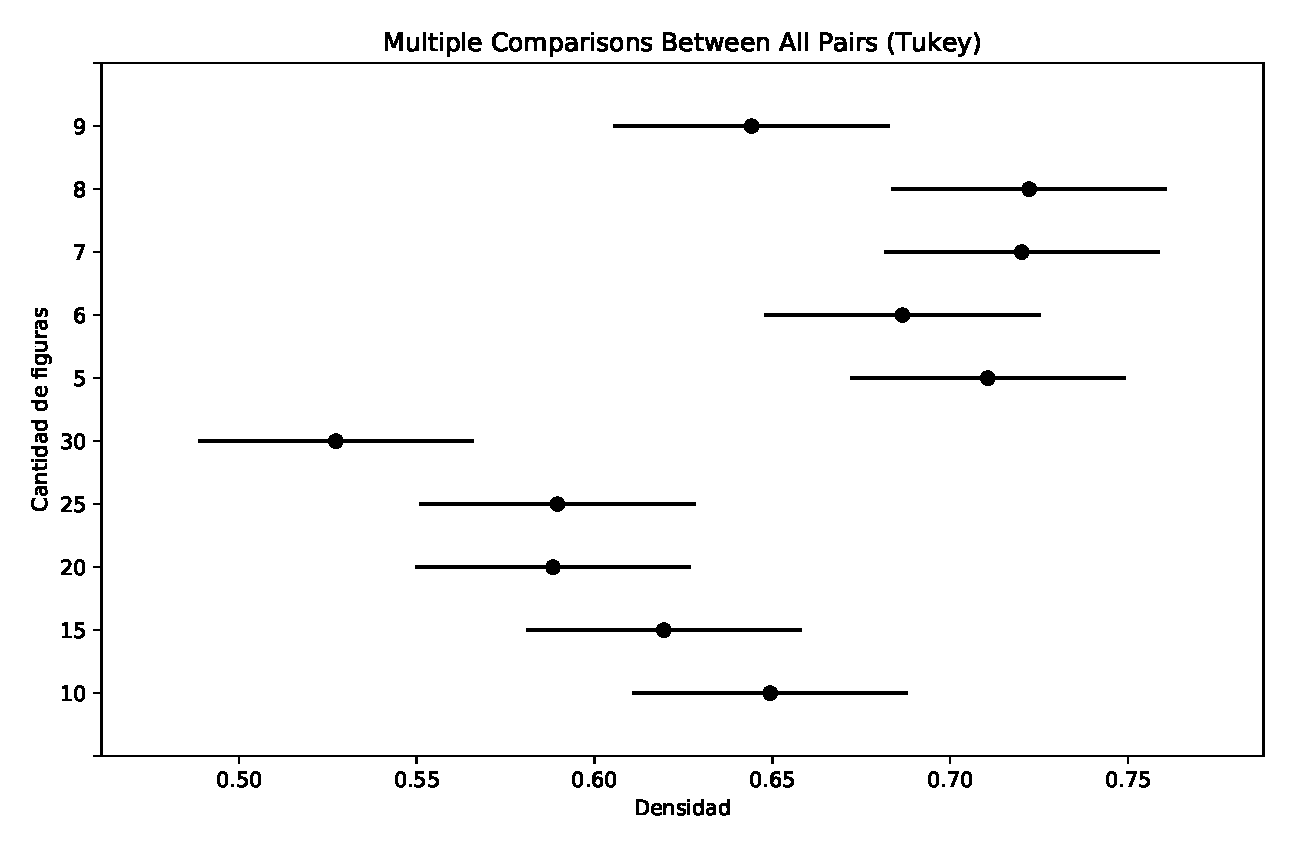
\includegraphics[scale=0.42, trim=8 8 8 20, clip=true]{figuras/simultaneous_tukeyCantidad_figuras.eps}
					\captionof{figure}{Diagrama simultaneo que relaciona el \% de ocupación del contenedor, con los grupos del factor cantidad de figuras}
					\label{fig:tykey1}
				\end{center}
			\end{figure}
		
\section{Análisis estadístico contenedor tipo circular} \label{Section5}

Para el análisis del los resultados obtenidos con el contenedor tipo circular se realiza el mismo procedimiento que en la sección \ref{Section4}.

Al realizar la prueba de Shapiro--Wilk, se obtiene un $\textbf{W}=0.928$ y un \textbf{valor $p$} = 0.001 mayor que $\alpha = 0.050$ por lo que existe suficiente evidencia para rechazar la hipótesis que la variable dependiente (densidad) sigue una distribución normal con un intervalo de confianza del 95\%. En la figura \ref{fig:normal2} se muestra que los puntos no se ajustan a lo largo de la línea de referencia, podemos asumir la falta de normalidad.
	\begin{figure}
				\begin{center}
					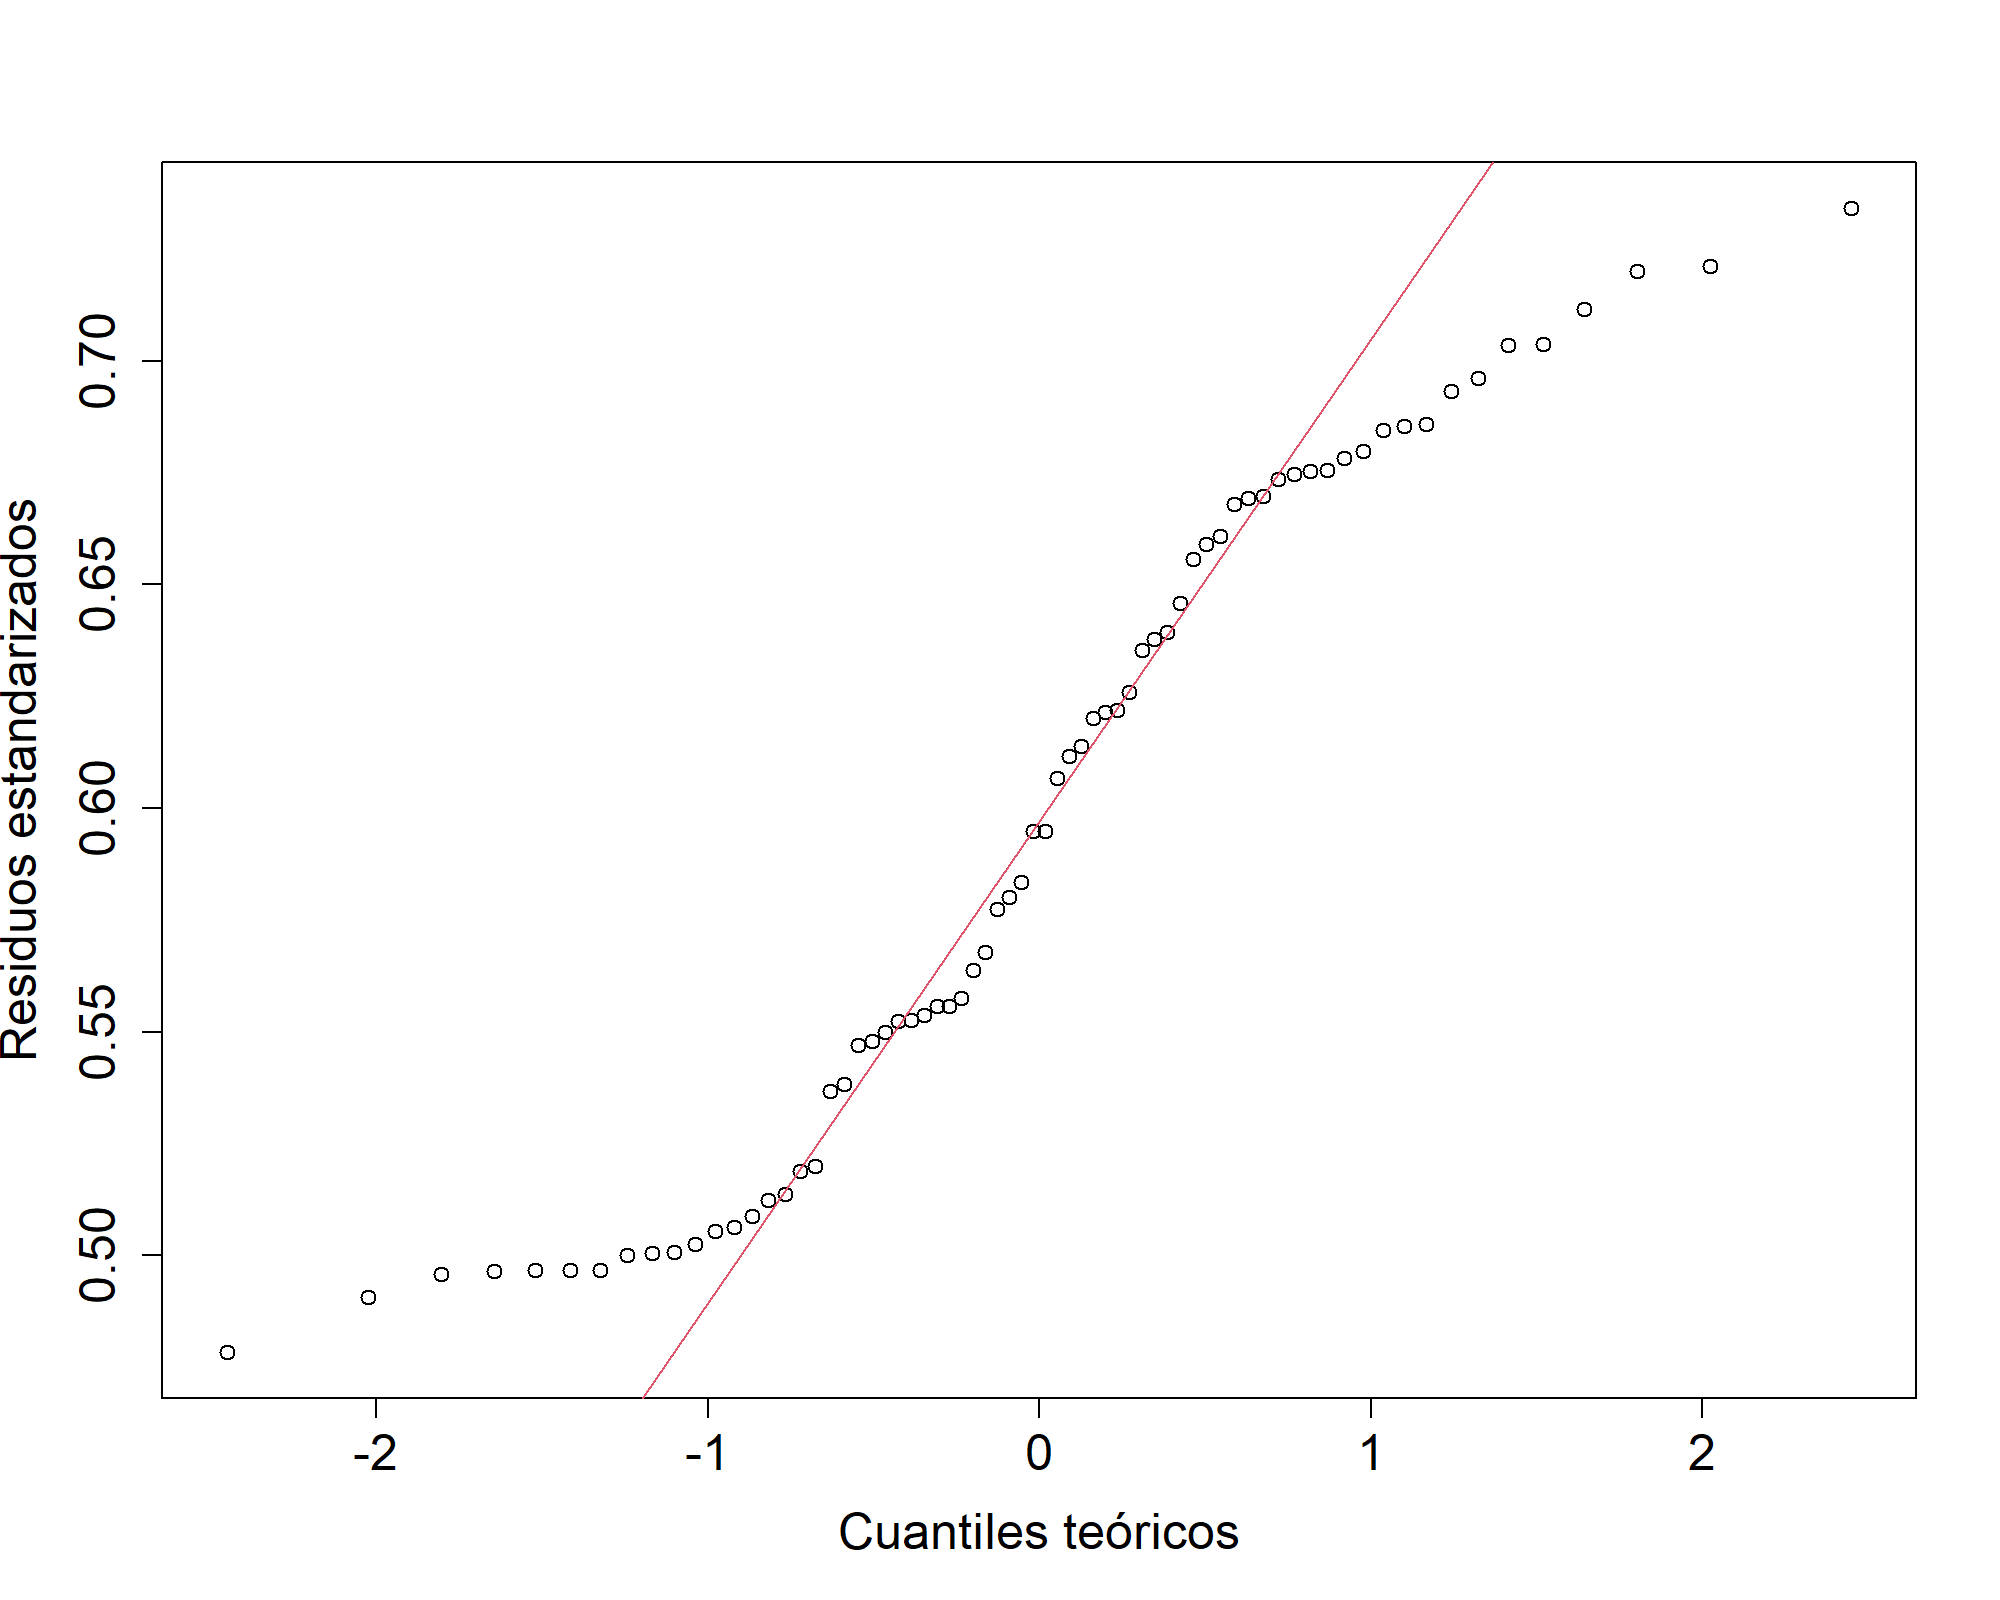
\includegraphics[scale=0.35]{figuras/circularnormal.png}
					\captionof{figure}{Gráfica Q-Q normal para la variable densidad}
					\label{fig:normal2}
				\end{center}
			\end{figure} 

Dado que los valores de la variable dependiente no siguen una distribución normal, se procede a aplicar la prueba H de Kruskal-Wallis que es una versión no paramétrica de ANOVA. En este caso se plantea la interrogante: ¿Existe diferencias en el \% de ocupación según el tipo de figuras?

Según los datos obtenidos en la prueba, con un valor del estadístico de prueba $\textbf{H} = 9.639$ y \textbf{valor $p$} = 0.086 mayor que $\alpha = 0.050$, no existe evidencia suficiente para rechazar la nula, la cual indica que no existen diferencias estadísticamente significativas con un intervalo de confianza de un 95\%. Lo anterior se puede observar en la figura \ref{fig:boxplotc1}. 		
	\begin{figure}
				\begin{center}
					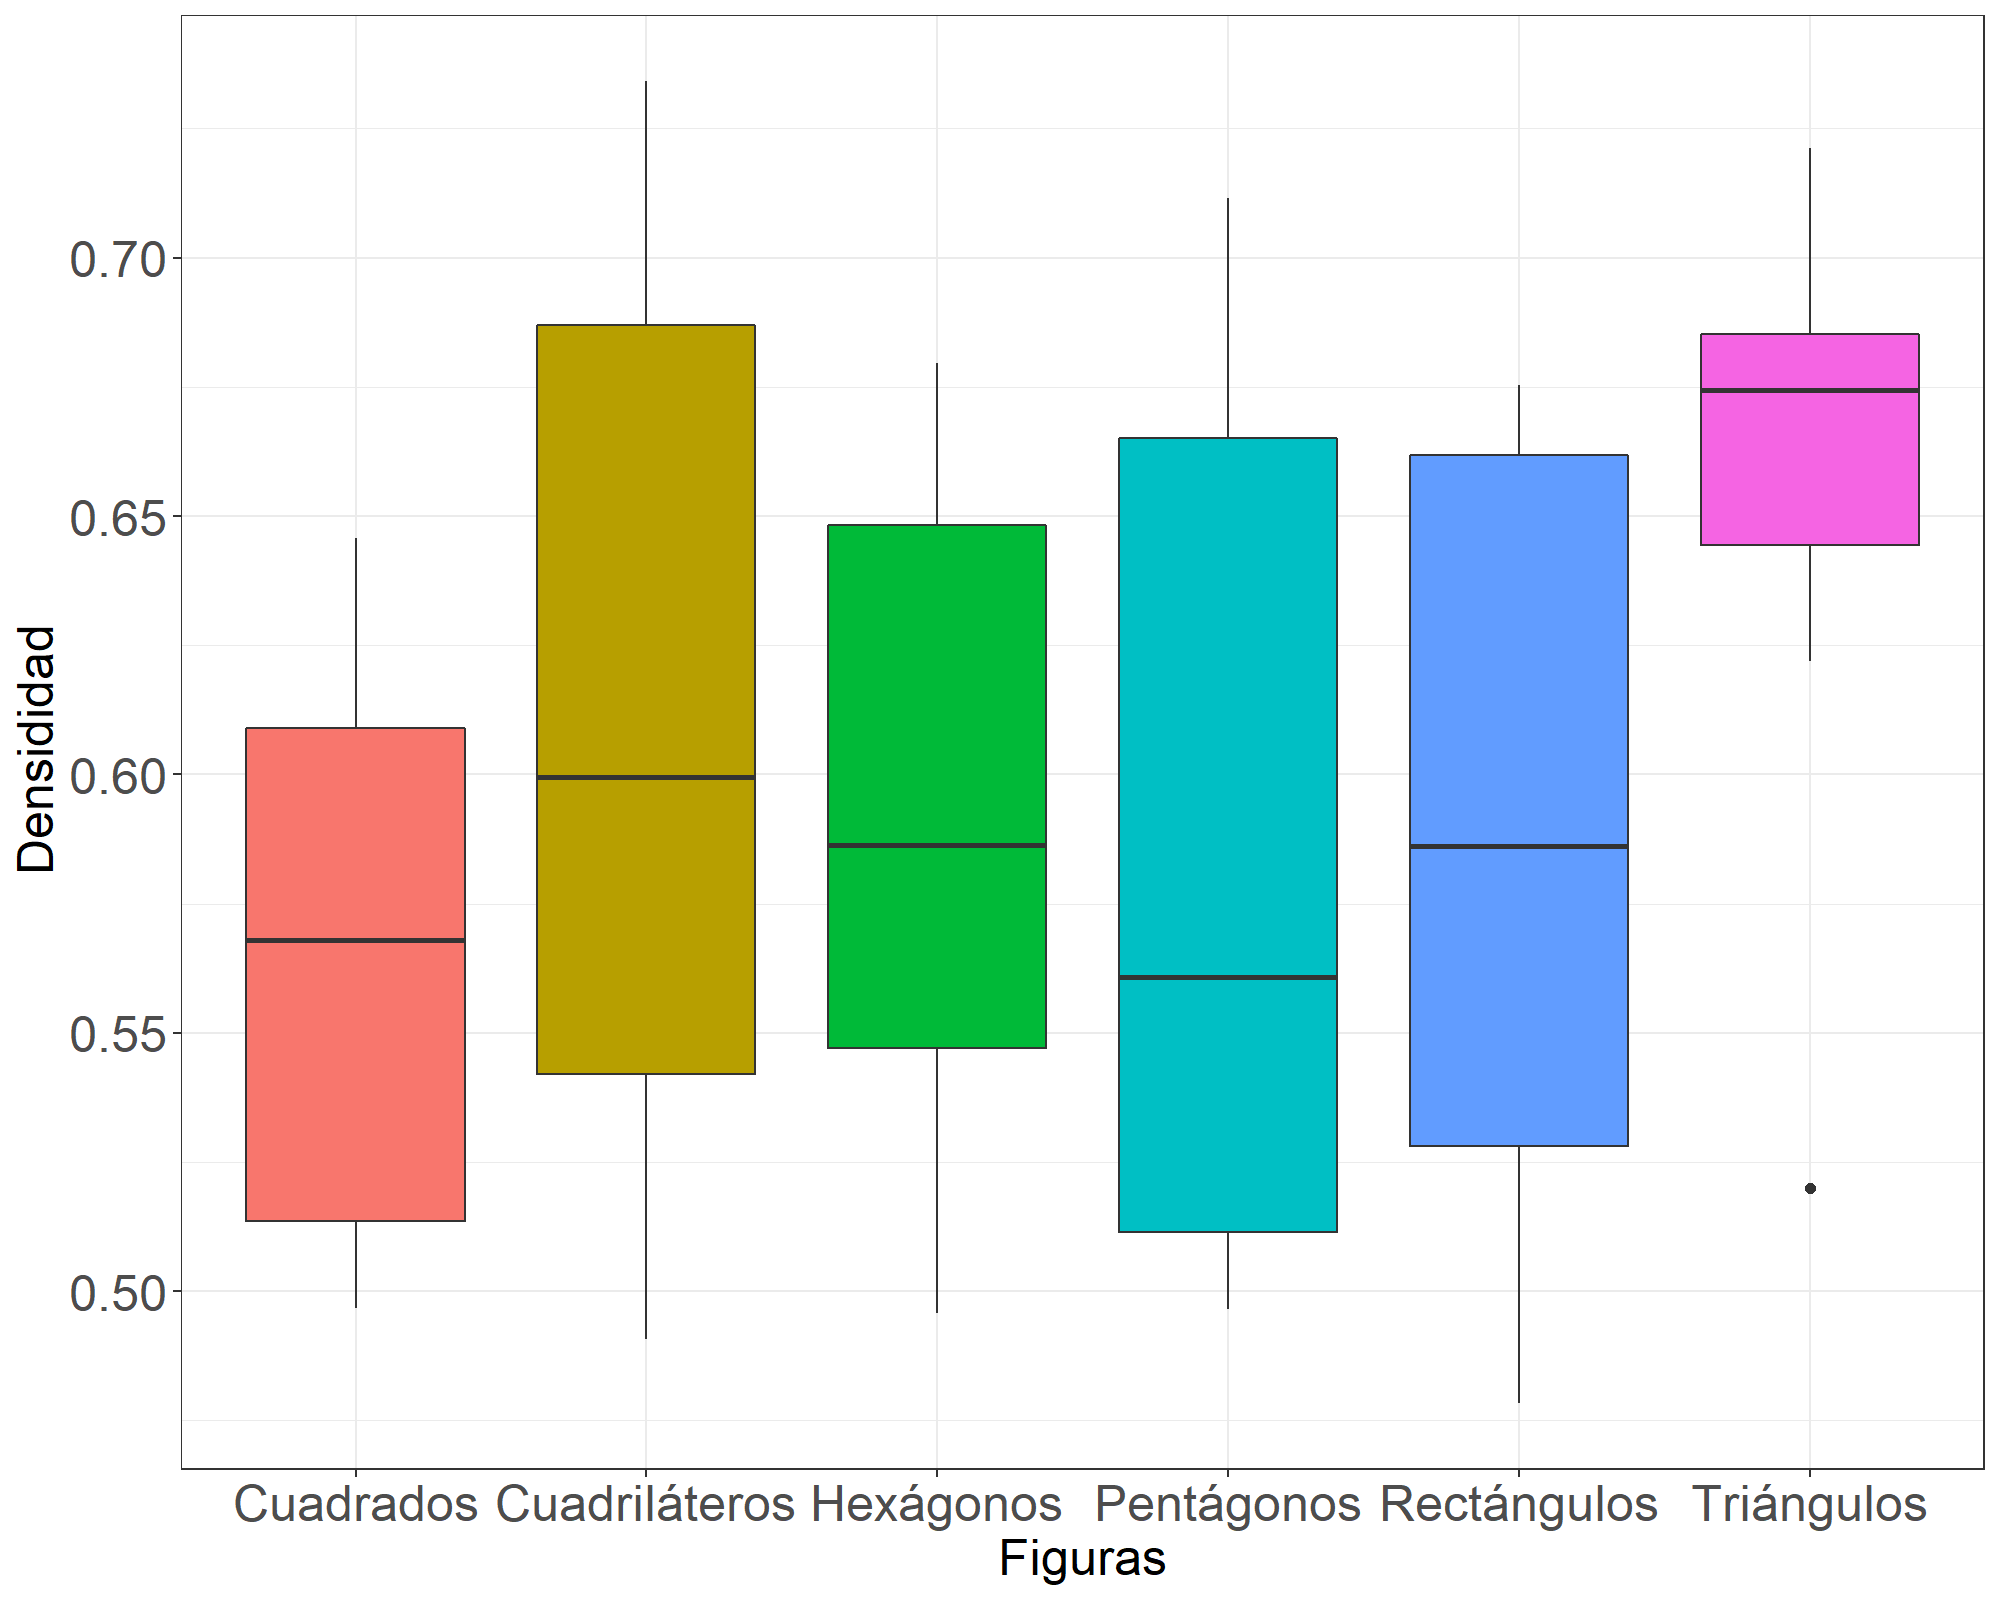
\includegraphics[scale=0.35]{figuras/Ccboxplot.png}
					\captionof{figure}{Diagrama de caja y bigotes que relaciona los tipos de figuras y el \% de ocupación del contenedor}
					\label{fig:boxplotc1}
				\end{center}
			\end{figure}
			
Para el factor cantidad de figuras se tiene como resultado de la prueba de Kruskal-Wallis un $\textbf{H} = 43.680$ y \textbf{valor $p$} = 0.000 menor que $\alpha = 0.050$, se tiene evidencia suficiente para rechazar la hipótesis $H_{0}$ ya que existe diferencias estadísticas significativas al menos entre dos de los grupos con un intervalo de confianza de un $95\%$, como se observa en la figura \ref{fig:boxplotc2}. 
	\begin{figure}
				\begin{center}
					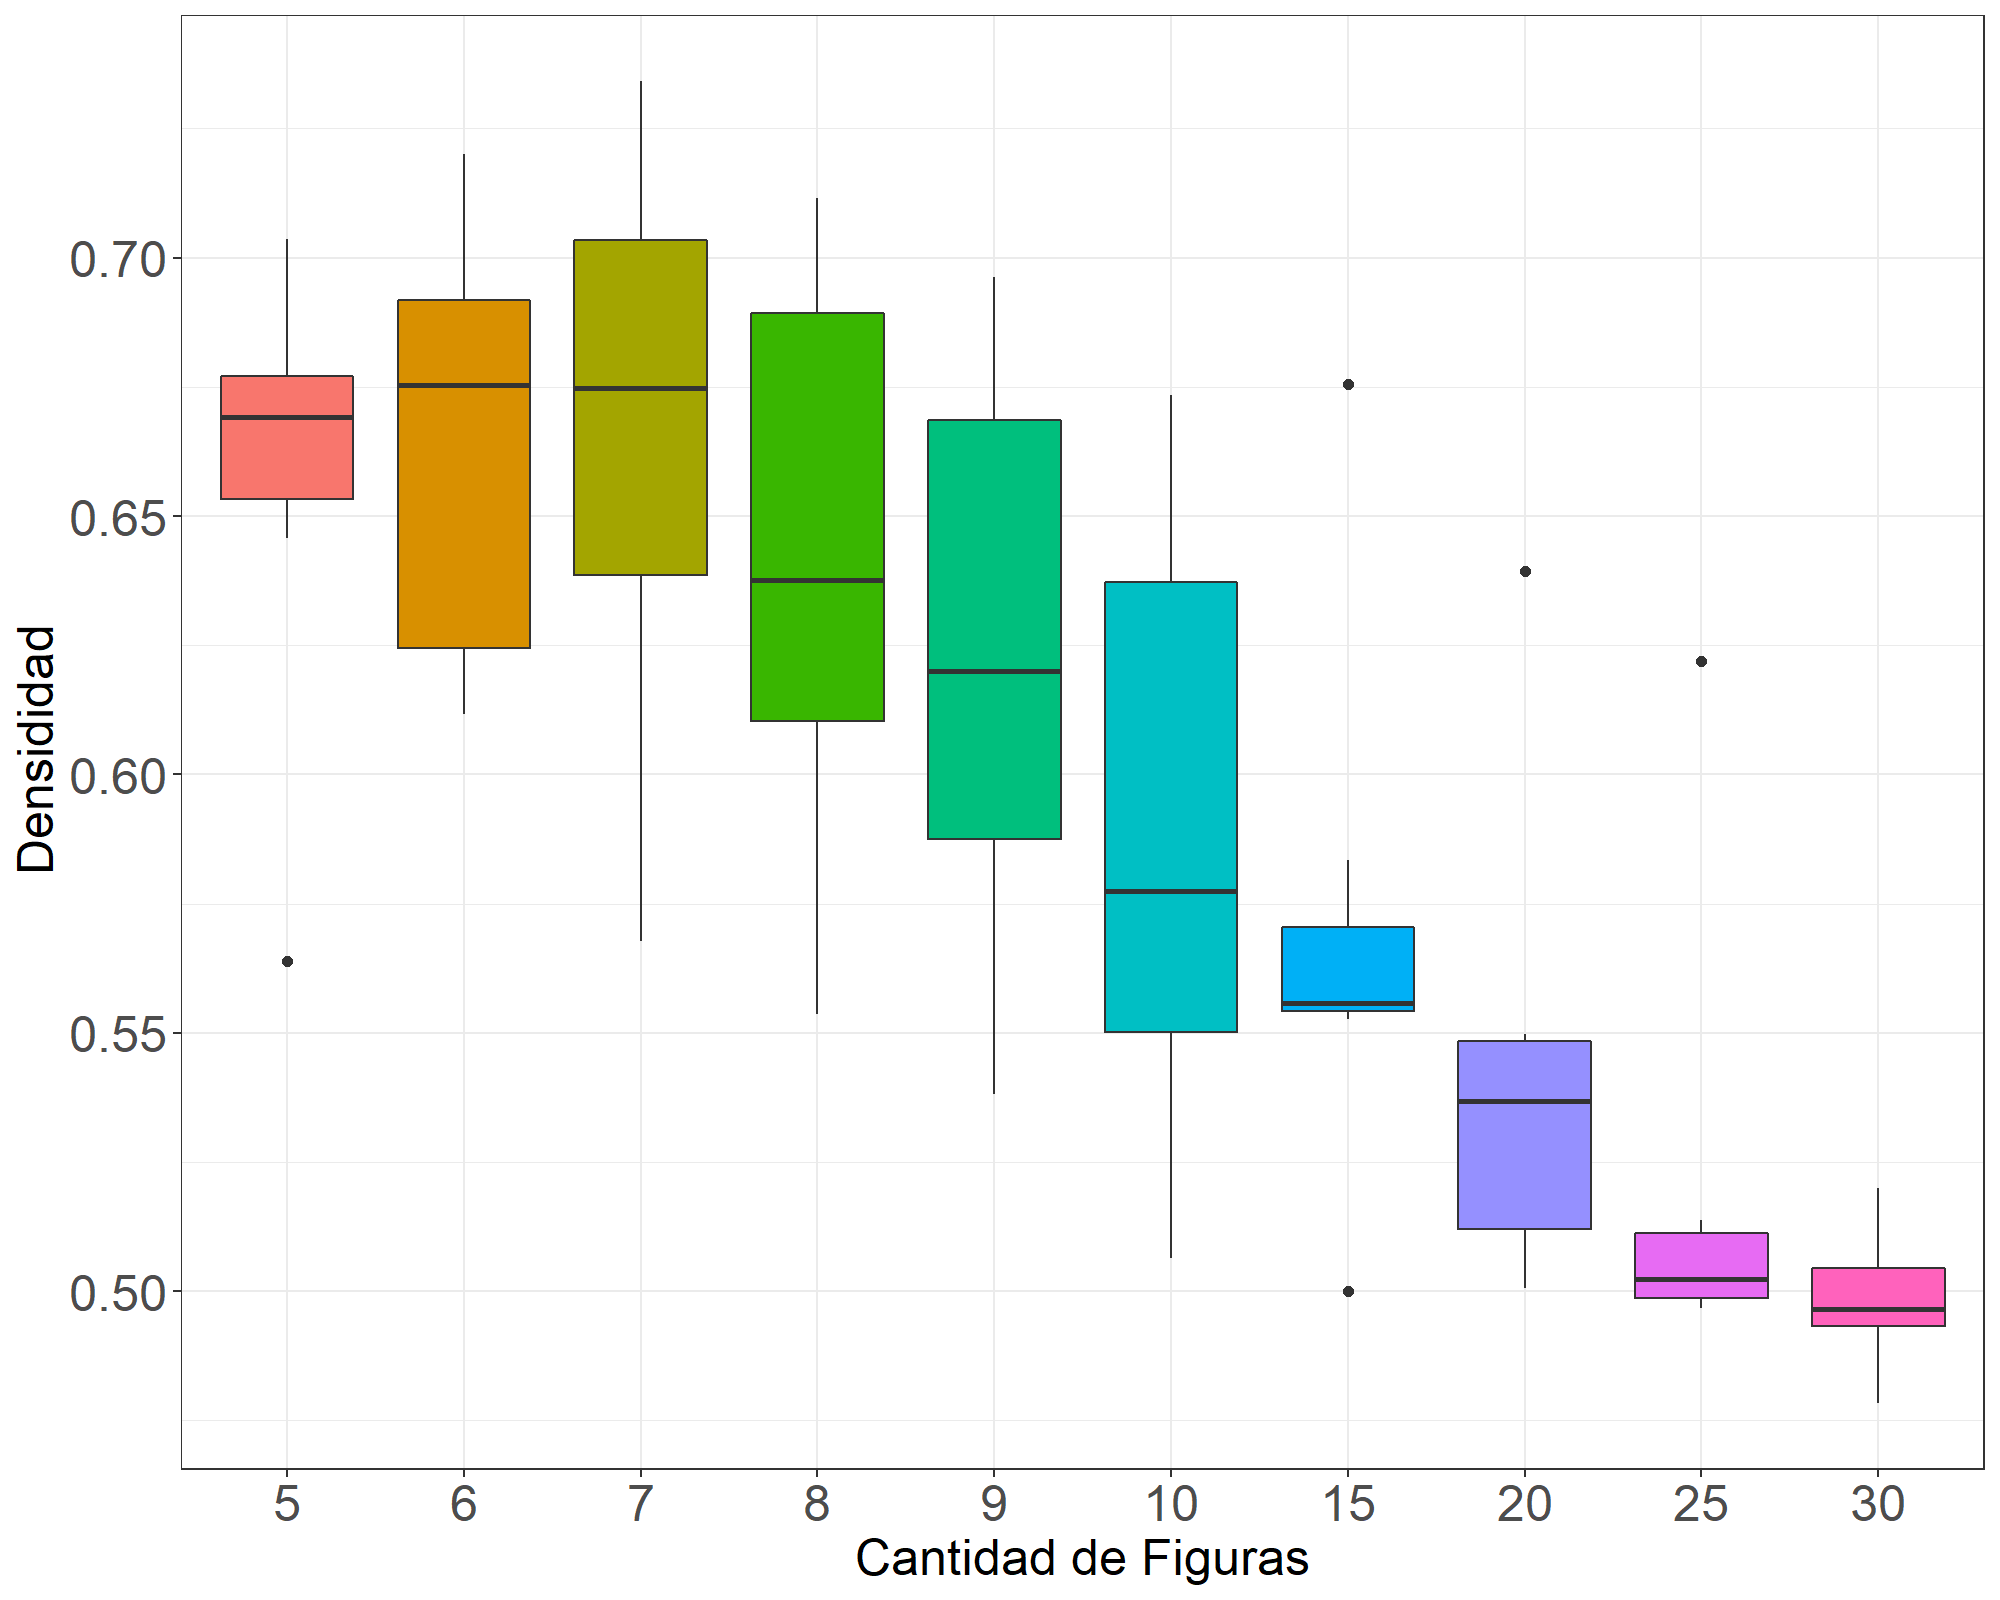
\includegraphics[scale=0.35]{figuras/Ceboxplotcant.png}
					\captionof{figure}{Diagrama de caja y bigotes que relaciona los cantidad de figuras y el \% de ocupación del contenedor}
					\label{fig:boxplotc2}
				\end{center}
			\end{figure}
			
Al igual que el ANOVA la prueba de Kruskal-Wallis no muestra entre que grupos existen las diferencias. Para saberlo es necesario compararlos todos con todos. Esto implica realizar una corrección del nivel de significancia para evitar incrementar el error de tipo I. El método de comparación \textit{post-hoc} que se utiliza para este caso es la prueba de rango de Tukey con la ficción \textit{kruskalmc()} de R \cite{R},  la cual arroja diferencias entre los grupos 5--25, 5--30, 6--25, 6--30, 7--25, 7--30, 8--30 y 9--30. Lo anterior viene dado por los \textbf{valores $p$} del pareo de esos grupos menores que $\alpha = 0.050$, por lo que se puede afirmar que existen diferencias estadísticamente significativas entre dichos grupos con un intervalo de confianza del 95\%. Gráficamente se puede ver en la figura \ref{fig:tykey2}.

	\begin{figure}
				\begin{center}
					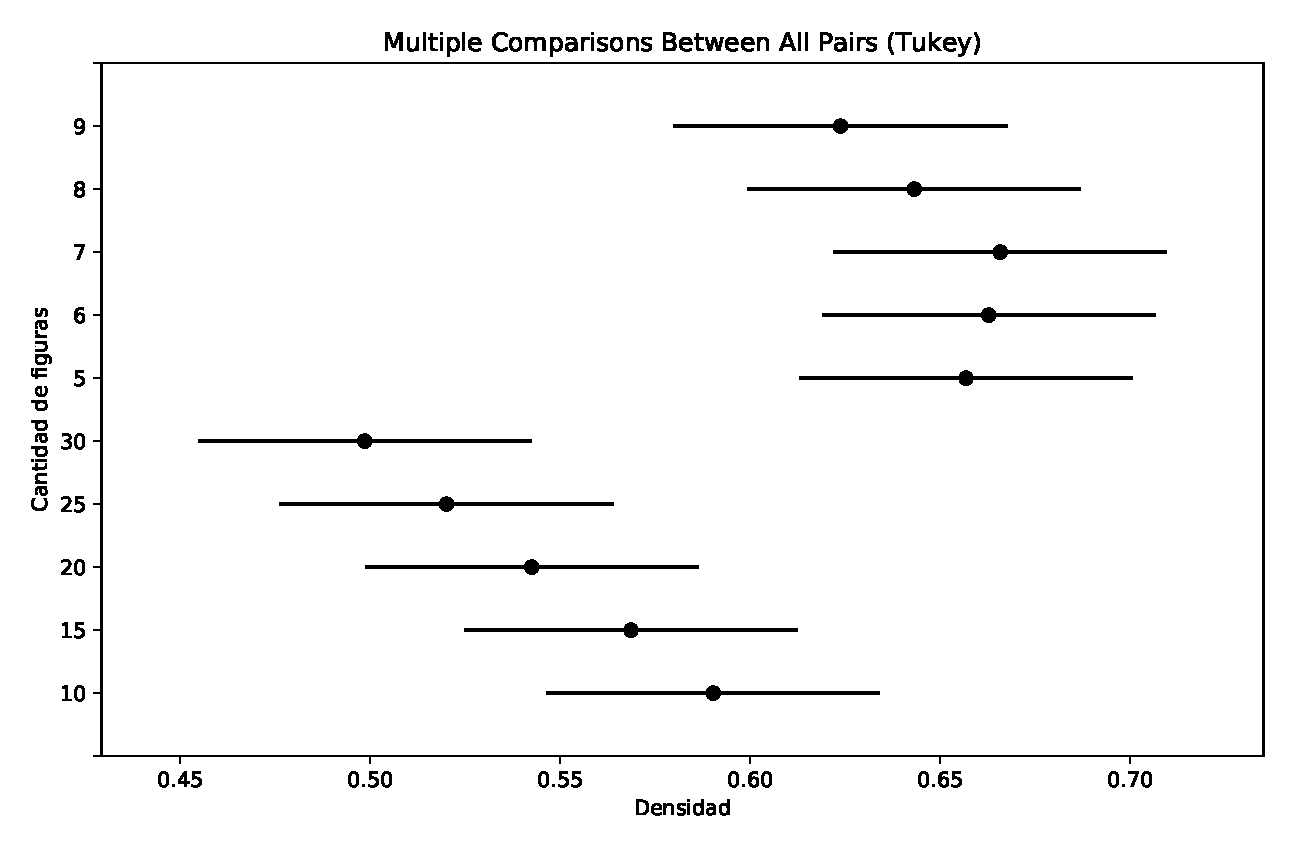
\includegraphics[scale=0.42, trim=8 8 8 20, clip=true]{figuras/simultaneous_tukeyCantidad_figuras1.eps}
					\captionof{figure}{Diagrama simultaneo que relaciona el \% de ocupación del contenedor, con los grupos del factor cantidad de figuras}
					\label{fig:tykey2}
				\end{center}
			\end{figure}
			
Se puede concluir de la aplicación de estas pruebas que el tipo de figura no influye significativamente en el porciento de ocupación del contenedor tipo circular. Además, se constató que el número de elementos a empacar si influye en dicho porciento.     
	
\section{Análisis estadístico según el tipo de contenedor}\label{Section6}
Con la aplicación de la prueba de Shapiro--Wilk a la variable dependiente, se obtiene un $\textbf{W}=0.955$ y un \textbf{valor $p$} = 0.000 menor que $\alpha = 0.050$ por lo que existe suficiente evidencia para rechazar la hipótesis que la variable sigue una distribución normal con un intervalo de confianza del 95\%.

Por lo que se aplica la prueba no perimétrica H de Kruskal-Wallis con el objetivo de conocer si el tipo de contenedor influye en la densidad del empaquetado. Con un estadístico de pruebas $\textbf{H}=12.727$	 y un \textbf{valor $p$} = 0.000 menor que $\alpha = 0.050$ se tiene evidencia para decir que el tipo de contenedor si influye en el porciento de ocupación con un intervalo de confianza del 95\%, ya que al solamente haber dos grupos no es necesario realizar la prueba \textit{post-hoc}. En la figura \ref{fig:boxplotcG}  se puede observar lo antes mencionado.   
	\begin{figure}
				\begin{center}
					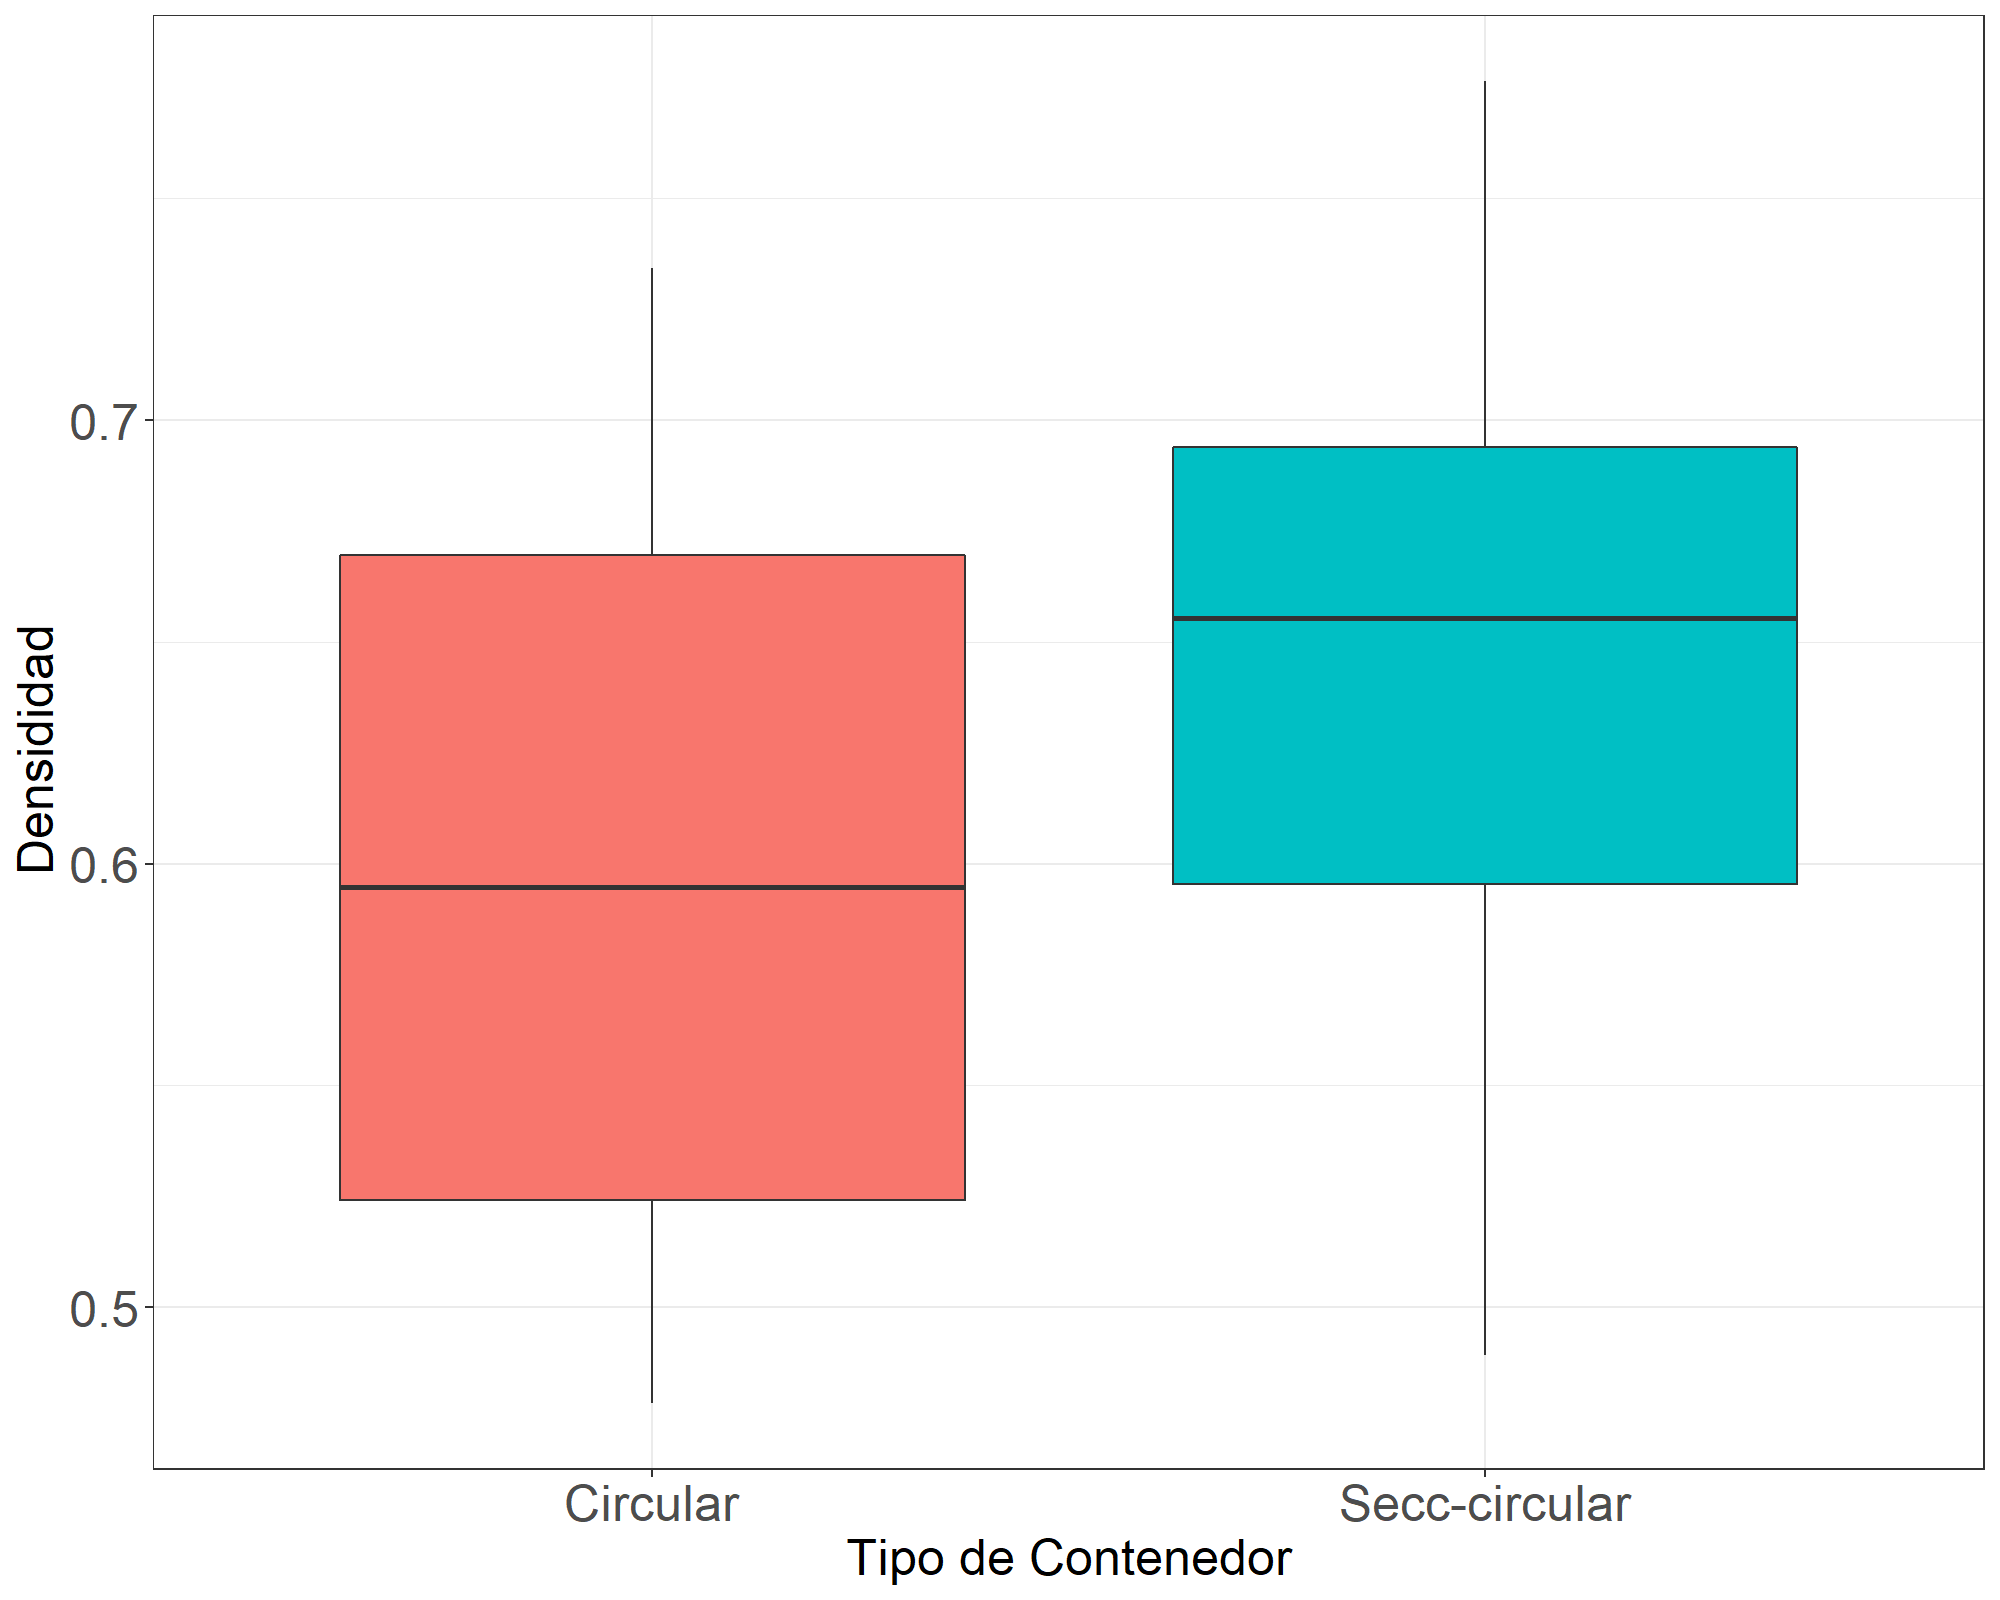
\includegraphics[scale=0.35]{figuras/Gboxplot.png}
					\captionof{figure}{Diagrama de caja y bigotes que relaciona los tipos de contenedores y el \% de ocupación del contenedor}
					\label{fig:boxplotcG}
				\end{center}
			\end{figure}
 
\section{Conclusiones} \label{Section7}
	
Los métodos estadísticos son muy útiles para poder comprender el comportamiento de los modelos, así como los factores que influyen en su desempeño. Con la aplicación de estos métodos en los resultados obtenidos mediante la experimentación computacional, se pudo identificar que el tipo de figuras a empaquetar no influye significativamente en la densidad de empaque para los dos tipos de contenedores analizados.

En el caso del factor cantidad de figuras se puede concluir que, para los dos tipos de contenedores dicho factor si influye en la densidad del empaque, comprobándose que para instancias más grandes las densidades disminuyen.

Además, se identificó que el tipo de contenedor también influye en el porciento de ocupación del contenedor para el modelo en cuestión.

%% If you have bibdatabase file and want bibtex to generate the
%% bibitems, please use
%%
\bibliographystyle{elsarticle-harv} 


%Offered Elsevier's bibliography styles that I could activate:
%% Numbered
%\bibliographystyle{model1-num-names}

%% Numbered without titles
%\bibliographystyle{model1a-num-names}

%% Harvard
%\bibliographystyle{model2-names}\biboptions{authoryear}

%% Vancouver numbered
%\usepackage{numcompress}\bibliographystyle{model3-num-names}

%% Vancouver name/year
%\usepackage{numcompress}\bibliographystyle{model4-names}\biboptions{authoryear}

%% APA style
%\bibliographystyle{model5-names}\biboptions{authoryear}

%% AMA style
%\usepackage{numcompress}
%\bibliographystyle{model6-num-names}

%% `Elsevier LaTeX' style
%\bibliographystyle{elsarticle-num}

\bibliography{biblio}
\end{document}
